\chapter{Implementierung}




\section{Softwaredokumentation}
\subsection{Bibliothek Keys}
\begin{figure}
  \centering
  %\includegraphics[angle=90,width=1\textwidth]{images/diagram_keys.png}
  \caption{Aktivitätsdiagramm für die Bibliothek Keys}
  \label{diagram_keys}
\end{figure}

\subsection{Software auf dem Mikrocontroller}
\begin{figure}
  \centering
  %\includegraphics[angle=90,width=1\textwidth]{images/diagram_arduino.png}
  \caption{Aktivitätsdiagramm für die Software auf dem Mikrocontroller}
  \label{diagram_arduino}
\end{figure}



\section{Aufbau der Elektronik}
Verwendete Kabel \cite{ps2male} \cite{ps2female}, Arduino Mega und Ethernet \cite{arduino} und PS/2-Tastatur.
\begin{figure}
  \centering
  \begin{minipage}{0.45\textwidth}
    \centering
    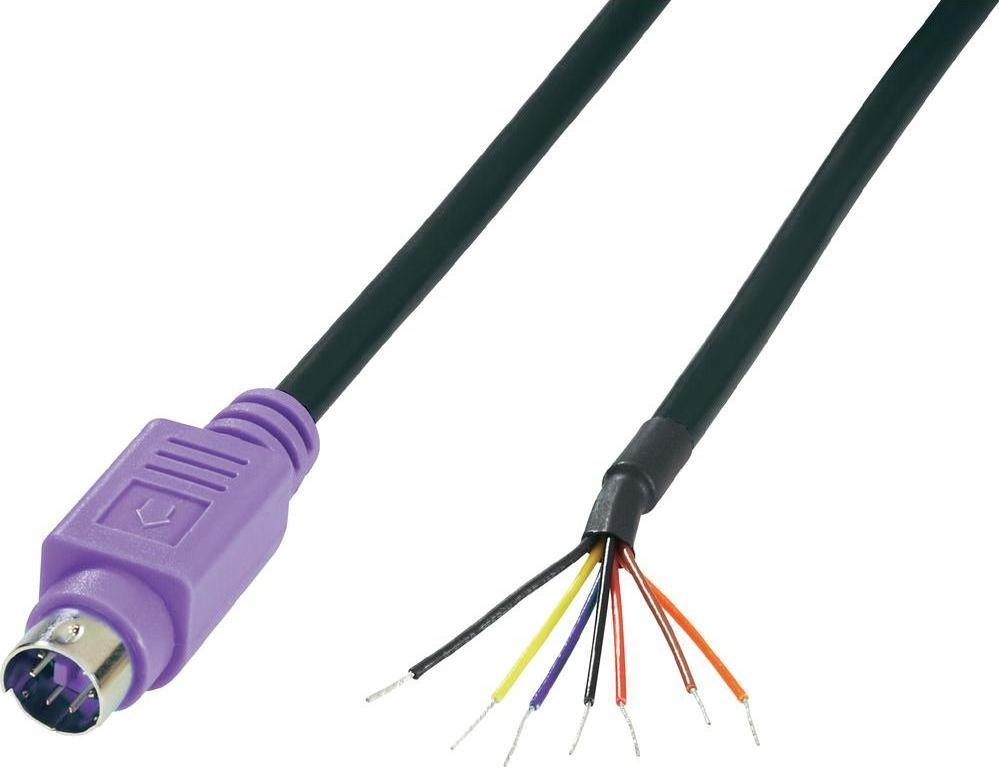
\includegraphics[width=1\textwidth]{images/ps2_male.jpg}
    \caption{PS/2 Male}
    \label{ps2_male}
  \end{minipage}
  \begin{minipage}{0.45\textwidth}
    \centering
    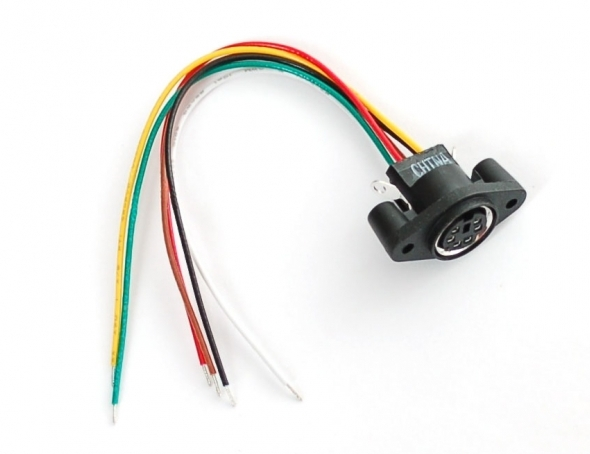
\includegraphics[width=1\textwidth]{images/ps2_female.jpg}
    \caption{PS/2 Female}
    \label{ps2_female}
  \end{minipage}
\end{figure}

\begin{figure}
  \centering
  %\includegraphics[width=0.8\textwidth]{images/hall_effect_sensor.jpg}
  \caption{Schema des Aufbaus fritzing}
  \label{fritzing}
\end{figure}

\begin{figure}
  \centering
  %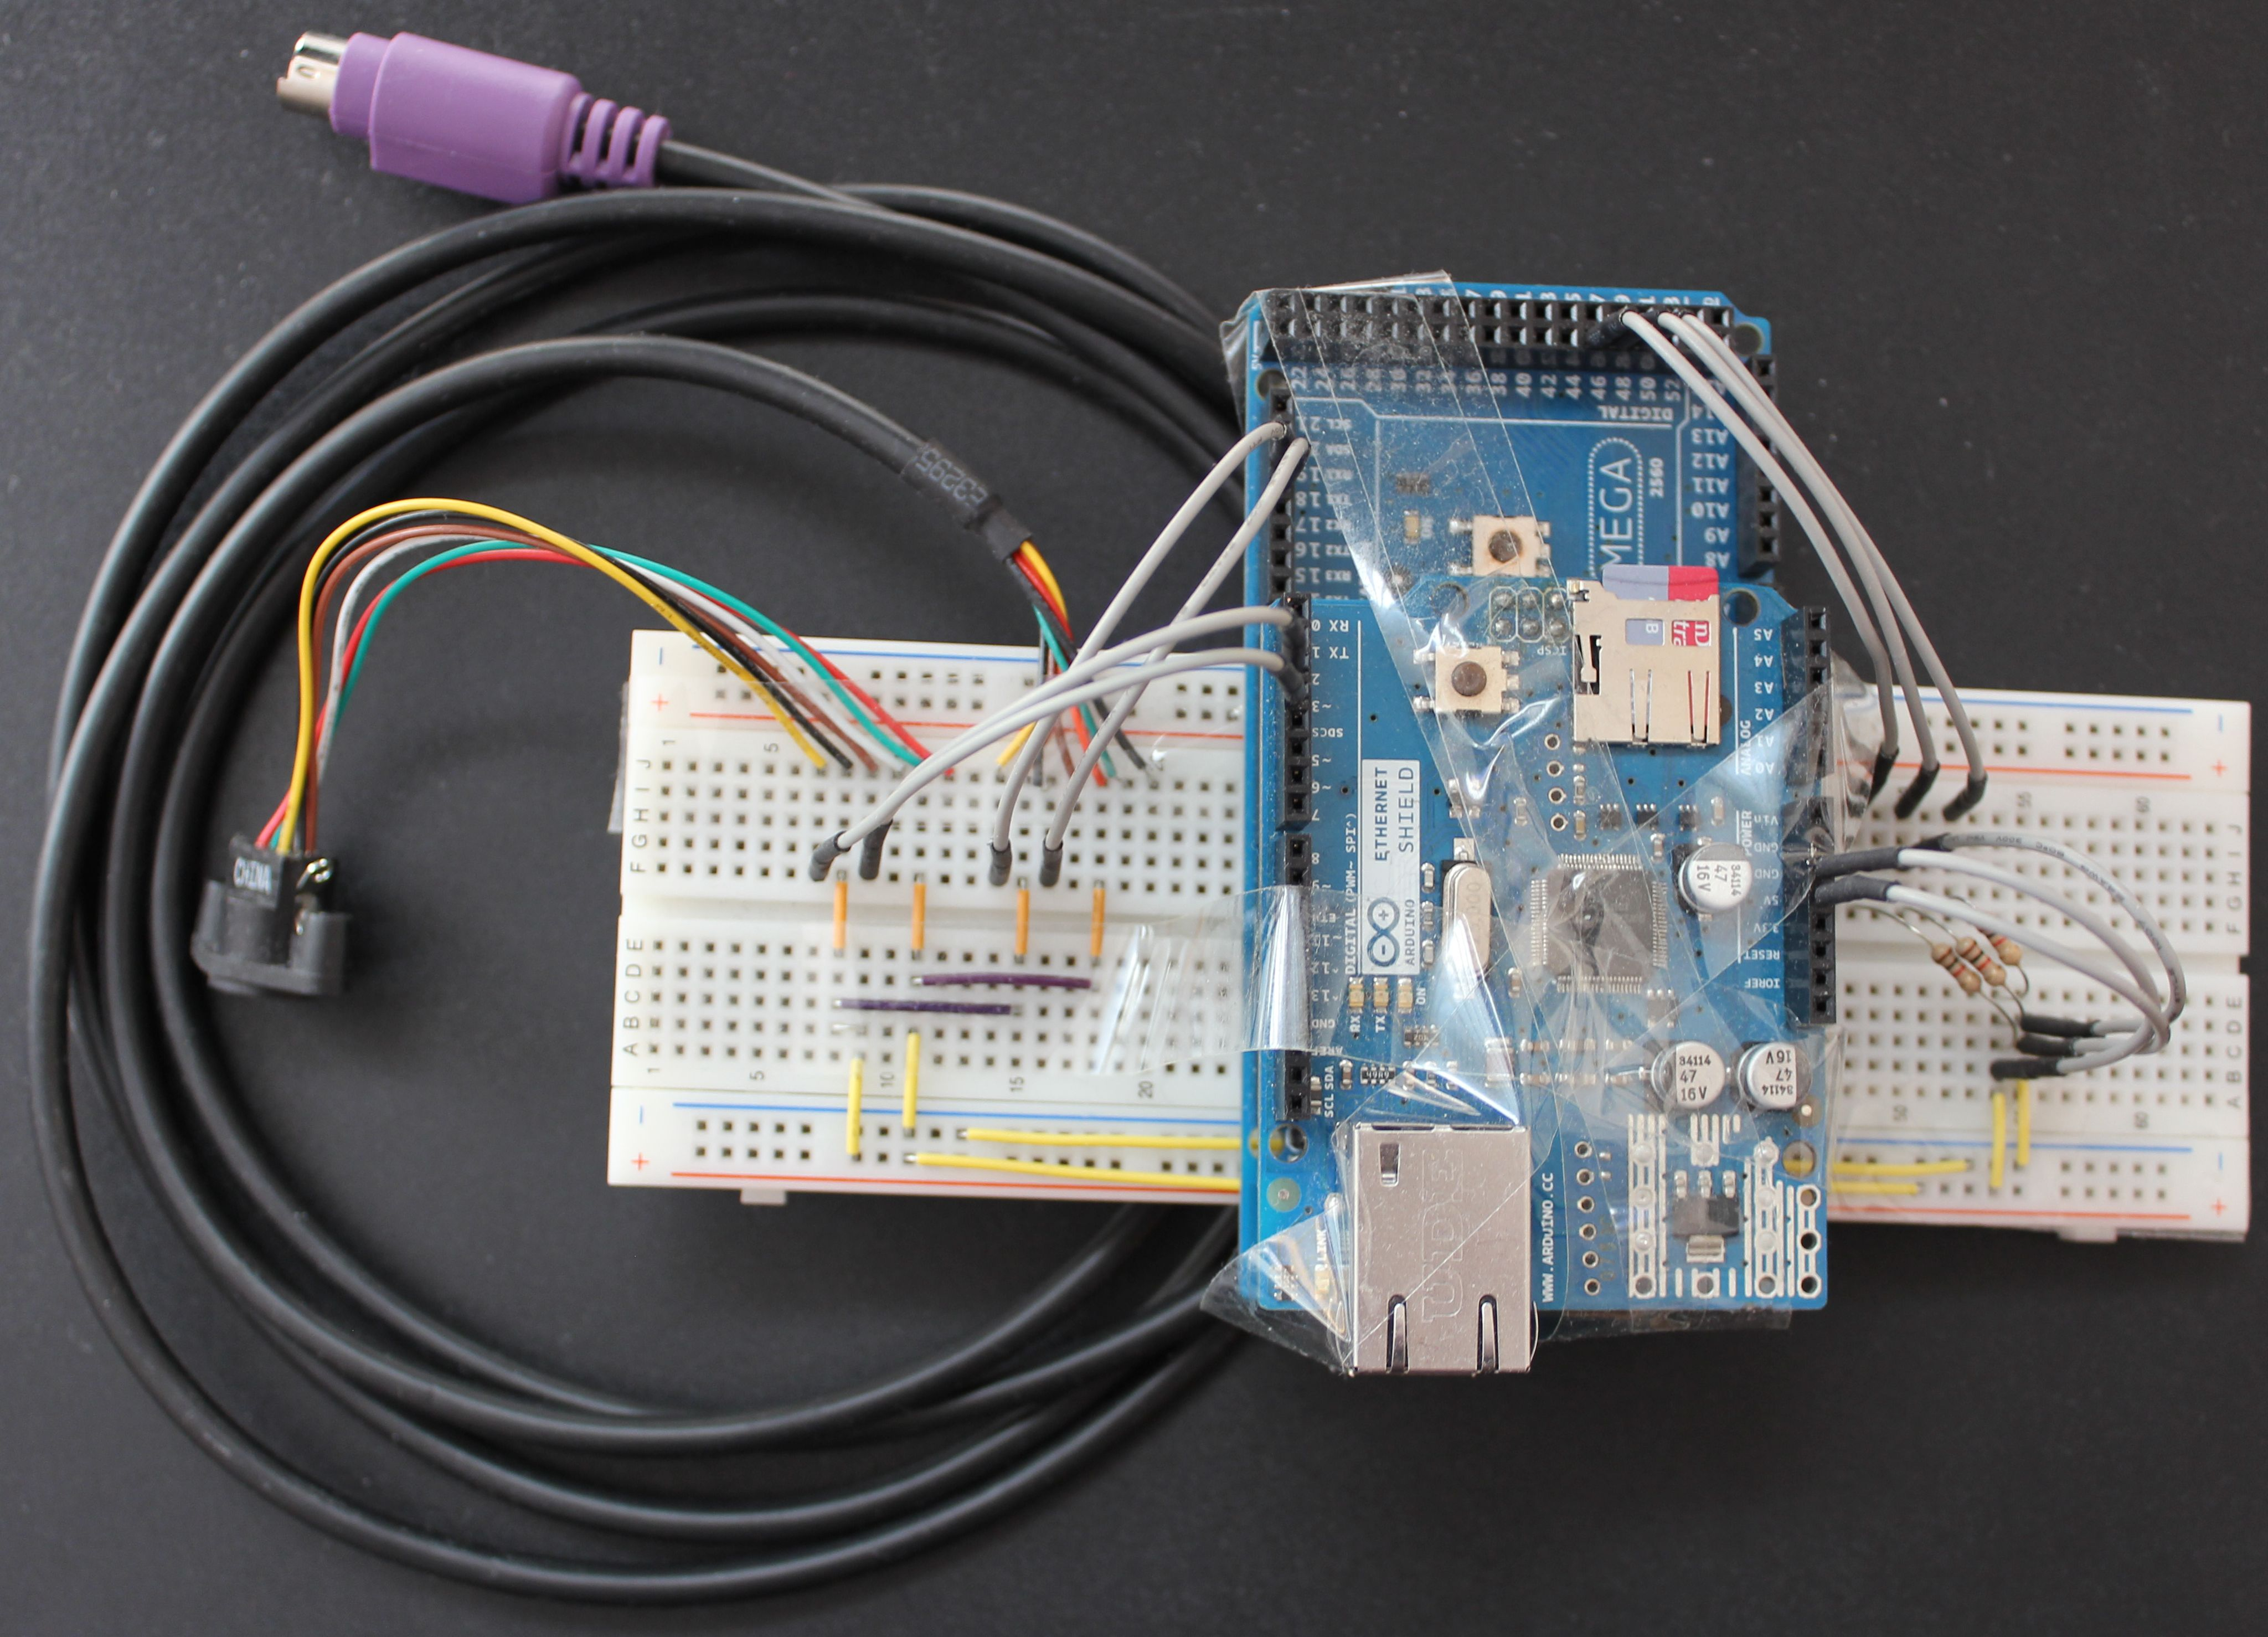
\includegraphics[width=0.8\textwidth]{images/foto1.jpg}
  \caption{Foto des Arduino Ethernet Shields und des Mega 2560 Boards}
  \label{foto1}
\end{figure}